% Metódy inž7inierskej práce

\documentclass[10pt,oneside,slovak,a4paper]{article}

\usepackage[slovak]{babel}
%\usepackage[T1]{fontenc}
\usepackage[IL2]{fontenc} % lepšia sadzba písmena Ľ než v T1
\usepackage[utf8]{inputenc}
\usepackage{graphicx}
\usepackage{url} % príkaz \url na formátovanie URL
\usepackage{hyperref} % odkazy v texte budú aktívne (pri niektorých triedach dokumentov spôsobuje posun textu)

\usepackage{cite}
%\usepackage{times}

\pagestyle{myheadings}

\title{Možnosti a efektívnosť získania jazykových znalostí prostredníctvom
e-learningu\thanks{Semestrálny projekt v predmete Metódy inžinierskej práce, ak. rok 2020/21, vedenie: Ing. Fedor Lehocki }} % meno a priezvisko vyučujúceho na cvičeniach

\author{Richard Szarka\\[2pt]
	{\small Slovenská technická univerzita v Bratislave}\\
	{\small Fakulta informatiky a informačných technológií}\\
	{\small \texttt{xszarkar@stuba.sk}}
	}

\date{\small 7. október 2020} % upravte



\begin{document}

\maketitle

\begin{abstract}
Získavanie vedomostí cez internet je čoraz bežnejšie. Jednou z najžiadanejších oblastí v e-learningu je najmä získavanie jazykových znalostí. Na osvojenie si jazyka v kontaktnom vzdelávaní je potrebné precvičovať jazyk rôznymi metódami rovnako ako pri autonómnom vzdelávaní pomocou e-learningu. Cieľom tejto práce je definovať a porovnať metódy nadobúdania jazykových zručností prostredníctvom e-learningu. V práci si rozoberieme metódy, ako úlohy zadávané softwarom (Duolingo), aktívnu komunikáciu s osobou, ktorá daný jazyk už ovláda (Tandem, HelloTalk) alebo pasívnu komunikáciu so skupinou ľudí s rovnakým cieľom (jazykové blogy). Zameriame sa na to, aké výhody i nevhody majú jednotlivé metódy a aká je efektívnosť nadobúdania jazykových znalostí cez e-learning.
\end{abstract}

\section{Úvod} %1 uvod
V súčastnosti nastal veľký rozmach v oblasti vzdelávania jazykových zručností prostredníctvom e-learningu. Mobilné aplikácie a jazykové blogy s stali veľmi obľúbenými najmä u mladých ľudí, a to predovšetkým vďaka svojej atraktivite jednoduchosti používania a možnosti motivácie.

Prekladaná práca pozostáva z 5 kapitol. V druhej kapitole si zadefinujeme pojem e-lerning a bližšie sa zameriame na jeho výhody a nevýhody. V tretej kapitole si rozoberieme najznámejšie a najoblúbenejšie aplikácie a formy vzdelávania sa v jazykoch. Konkrétne sa budeme venovať aplikácii Duolingo, HelloTalk, Tandem a jazykovým blogom. 4. kapitola slúži na posúdenie efektívnosti  e-learningu pri jazykovom vzdelávaní. Predmetom tejto kapitoly bude štúdia uskutočnená na Katedre Anglického vzdelávania Univerzity Borneo v Tarakane, ktorá skúmala vplyv aplikácie Duolingo na zlepšenie slovnej zásoby u 19-tich študentov po dobu 30 dní.

Hlavným cieľom predkladanej práce je porovnať najznámejšie možnosti vzdelávania sa v oblasti jazykov a posúdenie ich efektívnosti.

\section{Čo je e-learning?}%2
Učenie sa v dnešnej dobe je tak jednoduché, že naň stačí použiť hocijaké komunikačné zariadene, ktoré je schopné dávať informácie\cite{vyhody}.Pod pojmom e-learning rozumieme vedomé použitie kominikačných a sieťových technológií v učení a učení sa. Alternatívnou definiciou e-learningu môže byť aplikovanie elektronických systémov, ako internet a počítače, ktoré šetria čas aj financie \cite{efektivnost}. 

\subsection{Výhody e-learningu}%2.1
Ku každej novej technológii patria výhody, tak ako aj nevýhody. V prvej podkapitole sa zameriame na výhody e-learningu v učení a výučbe, ktoré zahrňujú aj výučbu jazykov. Medzi tie patrí najmä to, že:
\begin{itemize}
\item e-learning je rýchly, dynamický a znižuje výdavky (ako napríklad cestovanie), \cite{efektivnost}
\item lekcie sú pripravované rôznymi učiteľmi, \cite{efektivnost}
\item interaktívne cvičenia zvyšujú motiváciu študentov, \cite{vyhody}
\item aktivity e-learningu prinášajú rozličné skúsenosti rôznym ľuďom a takéto aktivity pomáhajú tiež ľahšiemu učeniu, \cite{vyhody}
\item je to druh kooperatívneho vzdelávania. \cite{efektivnost}
\end{itemize}

\subsection{Nevýhody e-learningu}%2.2
V druhej podkapitole sa budeme venovať nevýhodám jazykového vzdelávania prostredníctvom e-learningu. Medzi ne môžeme zaradiť napríklad:

\begin{itemize}
\item jazykové a kultúrne rozdiely, \cite{efektivnost}
\item technologické problémy u študentov, ako technofóbia či  nedostupnosť požadovaných technológií, \cite{nevyhody}
\item znížená sociálna a kultúrna interakcia, ako je napríklad reč tela, \cite{nevyhody}
\item technické limitácie.\cite{efektivnost}
\end{itemize}

\section{Najznámejšie a najobľúbenejšie e-learningové možnosti učenia sa jazyka}%3
Najväčší rozmach získavania jazykových vedomostí zažívajú v dnešnej dobe hlavne rôzne mobilné aplikácie. Mnohé z nich sú považované za edukatívne hry, ako napríklad Duolingo. Atraktivita týchto aplikácií spočíva v ľahkej dostupnosti a v tom, že ich používanie je dostupné zadarmo, s výnimkou občasných reklám a zakúpenia plnej (premium) verzie aplikácie. Avšak, v ústraní neostali ani jazykové blogy.

\subsection{Aplikácia Duolingo}%3.1
Duolingo je mobilná aplikácia na vzdelávanie jazykov. Jej používanie je jednoduché a je vhodná takmer pre všetky vekové kategórie\cite{duolingo}. Umožňuje získavanie jazykových znalostí pomocou rôznych kurzov. Užívateľ si vyberie jazyk, ktorým hovorí (ak je dostupný) a jazyk, ktorý by sa chcel naučiť, prípadne ten, v ktorom by sa chcel zdokonaliť. Aplikácia Duolingo momentálne ponúka 36 kurzov pre anglicky hovoriacich užívateľov. Ponuka sa bude líšiť v závislosti od materinského jazyka. Pre slovensky hovoriacich užívateľov napríklad nie je dostupný žiadny kurz a pre českých uživateľov disponuje Duolingo iba kurzom anglického jazyka. Ak si ako jazyk, ktorému rozumiete, vyberiete nemčinu, tak máte na výber 4 kurzy(\href{https://www.duolingo.com/courses}{www.duolingo.com/courses}).

Aplikácia postupne pridáva nové kurzy a aktívne zveľaduje obsah, čím zvyšuj svoj dosah i atraktivitu pre potenciánych užívateľov. Pre porovnanie, v roku 2012 poskytovalo Duolingo len 5 kurzov a v roku 2020 celkovo až 95 (\href{https://www.businessofapps.com/data/duolingo-statistics/}{www.businessofapps.com/data/duolingo-statistics}) Tento vývoj môžeme vidieť aj na množstve aktívnych užívateľov aplikácie \ref{duo-uzivatelia}.

\begin{figure}[h] %obrázok
\centering
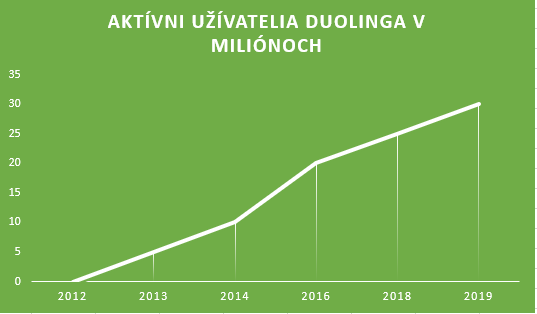
\includegraphics[width=\textwidth]{duolingo.png}
\caption{ Aktívni užívatelia aplikácie Duolingo v miliónoch.
Zdroj: \href{https://www.businessofapps.com/data/duolingo-statistics/}{www.businessofapps.com/data/duolingo-statistics}}
\label{duo-uzivatelia}
\end{figure}

Na grafe vidíme, že v roku 2012 bola aplikácia sprístupnená verejnosti. Rok na to (2013) bol počet aktívnych užívateľov na úrovni 5 miliónov. V roku 2014 sa množstvo aktívnych užívateľov zdvojnásobilo na 10 miliónov. O 2 roky neskôr (2016) ich bolo už 20 miliónov. V ďalších rokoch (2018, 2019), že pribudlo v oboch prípadoch 5 miliónov aktívnych užívateľov.

Pomerne novou funkciou na rozvoj jazykových zručností je sekcia "Duolingo stories". (\href{https://www.duolingo.com/stories/}{www.duolingo.com/stories}). V krátkych príbehov, v ktorých musí užívateľ zadávať gramaticky správne odpovede alebo vybrať odpoveď, ktorá sa hodí do daného kontextu. Veľkou výhodou tejto formy vzdelávania je udržanie pozornosti pomocou nepredvídateľných a zaujímavých koncov príbehov. 

\subsection{Aplikácia HelloTalk} %3.2
HelloTalk je populárny na trhu aplikácií na vzdelávanie jazyka. jeho hlavnou myšlienkou je prepojenie užívateľa, ktorý sa chce naučiť cudzí jazyk s osobou, ktorej je daný jazyk materisnký. HelloTalk disponuje množstvom rôznych funkcií. Niektoré z nich sa odomknú až po zakúpení prémium verzie. Podľa webovej stránky HelloTalk má aplikácia až sedem miliónov užívateľov.\cite{hellotalk}\\
Aplikáciou môžete zdieľať hlasové správy, čety, mobilnú kameru, čmáranice, emotikony, GPS lokáciu či špecifické pomocné prvky na vzdelávanie jazyka (preklad, rozozanie hlasu, ...).\cite{hellotalk}\\\\
Výhody aplikácie HelloTalk:
\begin{itemize}
\item možnosť bezpatného hovoru,
\item automatické prekladanie konverzácie, čo zabezpečuje plynulosť koverzácie,
\item pomoc pri výslovnosti pri jazykoch, ktoré nepoužívaju latinskú abecedu.\cite{hellotalk}
\end{itemize}
Nevýhody aplikácie HelloTalk:
\begin{itemize}
\item nedostatočný systém na motivovanie užívateľa,
\item nie všetky funkcie su dostupné bez prémium verzie,
\item žiadna spätná väzba pre užívatelov o ich progese v učení,
\item informovanie o čase v krajine osoby, ktorej píšem (odpoveď na otázku, či je vhodné začať konverzáciu).\cite{hellotalk}
\end{itemize}
\subsection{Aplikácia Tandem} %3.3
Tandem je aplikácia založená na metóde výmeny jazykových znalostí, ktorá má korene v sedemdesiatych rokoch minulého storočia. Metológia vzdelávania aplikácie Tandem je založená na koncepte rozhovoru medzi dvomi Tandem partnermi, pričom ideálne je ak jeden z nich má daný jazyk ako materinský.

Zaujímavým prvkom tejto aplikácie je proces posúdenia nových uživateľov.\cite{tandem} Tandem je zameraný čisto na jazykové účely, a preto tento proces pomáha vyfiltrovať adeptov s inými zámermi. Proces posúdenia prebieha v podobe vyplnenia budúceho profilu užívateľa. Pri zadávaní profilovej fotografie vás aplikácia Tandem automaticky upozorní, ak fotografia nespĺňa požadované kritériá \ref{tandem-obmedzenia}. Čas čakania na odsúhlasenie sa líši. Niektorí užívatelia boli odsúhlasení za niekoľko dní, iní za zopár týždnov.

\begin{figure}[h] %obrázok
\centering

\includegraphics{tandem2.png}
\caption{Upozornenie po zadaní profilovej fotky, na ktorej nie je tvár. Zdroj: Vlastné spracovanie}
\label{tandem-obmedzenia}
\end{figure}

Tandem pozostáva z troch hlavných zložiek. Prvou je komunita, ktorá slúži na hľadanie vhodných Tandem partnerov. Keďže partneri sa nemôžu považovať za jazykových expertov, tak aplikácia umožňuje spojenie sa s platenými učiteľmi jazyka, čo je druhou zložkou. Poslednou sú čety, ktoré sú určené na prehľad a sumarizáciu konverzácií užívateľa.\\\\\\\\\\\\
Výhody aplikácie Tandem: 
\begin{itemize}
\item užívateľ si vie vybrať Tandem partnera podľa spoločných záujmov uvedených v profile,\cite{tandem}
\item Tandem partneri si vedia navzájom opraviť gramatiku prostredníctvom vstavanej funkcie,
\item Tandem umožňuje videochaty \cite{tandem} a audio-správy,
\item užívatelia môžu filtrovať to, kto vidí ich profil a prípadne prerušiť kontakt s nežiadúcou osobou. \cite{tandem}
\end{itemize}
Nevýhody aplikácie Tandem:
\begin{itemize}
\item užívateľ musí mať aspoň základné porozumenie jazyka, ináč sa s tandem partnerom nedorozumie (avšak môže využiť služby učiteľov), \cite{tandem}
\item veľa užívateľov využíva aplikáciu na zoznamovanie sa s novými ľuďmi, čo môže brániť vo vzdelávaní, \cite{tandem}
\item proces posudzovania profilu môže trvať dlho, veľa uživateľov sa na to sťažuje, \cite{tandem}
\end{itemize}

\subsection{Jazykové blogy} %3.4

Blogy a weblogy sú ľuďom známe už od vzniku svetovej počítačovej siete. Blogy sú online priestory na písanie, ktoré môžu byť upravené v okamihu a publikované verejne cez internetové prehliadače. Fungujú na princípe online denníkov, ktorých obsah autor môže aktualizovať obsah denne. V edukačnej sfére sú blogy veľmi  populárne, najmä u učitelov a žiakov pri učení sa jazyka. Tí sa o ne čoraz viac zaujímajú, pretože blogovanie sa zameriava na zdieľanie jednoduchého textu a vzájomného komentovania príspevkov. Používanie blogov sa stále považuje za relatívne novú metódu výučby a učenia sa cudzieho jazyka. \cite{blog-mif}\\
Vo svojej štúdii Miftachudin \cite{blog-mif} uvádza v sumarizácii 3 výhody a 3 nevýhody jazykových blogov.\\
\\
Výhody jazykových blogov:
\begin{itemize}
\item zlepšenie písacích schopností,
\item používanie blogov núti užívateľa čítať viac v danom jazyku,
\item blogy sú dobré médium na interakciu s ľudmi v danom jazyku. \cite{blog-mif}
\end{itemize}
Nevyhody jazykových blogov:
\begin{itemize}
\item chýba prvok na motivovanie užívateľov, čo vedie k nepravidelnému používaniu jazykových blogov,
\item niektorí užívatelia nemajú dosť sebaistoty na zdieľanie ich prác,
\item užívatelia môžu mať problém s porozumením inštrukcií na spravovanie blogu. \cite{blog-mif}
\end{itemize}



\section{Efektívnosť e-learningu pri jazykovom vzdelávaní}
V tejto sekcii si rozoberieme štúdiu zameranú na výskum efektivity jazykového vzdelávania prostredníctvom e-learningu. Konkrétne sa budeme venovať štúdii uskutočnenej na Katedre Anglického vzdelávania Univerzity Borneo v Tarakane.

\subsection{Vplyv Duolinga na slovnú zásobu}
V štúdii sa výsledky zlepšenia slovnej zásoby subjektov posudzovali pomocou testu na anglickú slovnú zásobu pred a po používaní aplikácie Duolingo. Subjektmi boli devätnásti študenti druhého semestra akademického roku 2018/2019 Katedry Anglického vzdelávania Unverzity Borneo v Tarakane. Ich úlohou bolo robiť zadania Duolinga, kým nedosiahli 20 bodov skúsenosti (body v Duolingu) po dobu 30 dní. Test pred aj po vyhradenej dobe pozostával z 25 otázok na slovnú zásobu. Výsledky testov môžeme vidieť na obrázku číslo \ref{duo-studium}. \cite{duolingo}

\begin{figure}[h] %obrázok
\centering
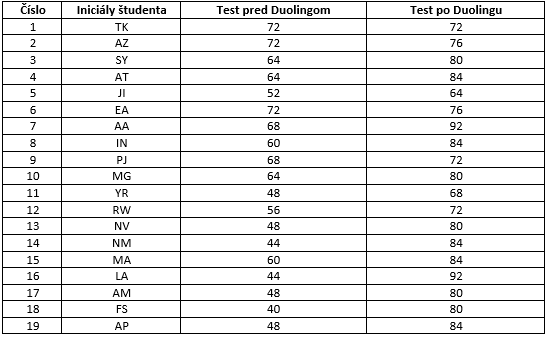
\includegraphics{duo_studium.png}
\caption{Výsledky pred a po používania aplikácii Duolingo\cite{duolingo}}
\label{duo-studium}
\end{figure}

V tabuľke \ref{duo-studium} pozorujeme, že najmenší počet bodov na teste pred používaním Duolinga je 44 a najväčší 72. Najmenší počet bodov na teste po používaní aplikácie  Duolingo po dobu 30 dní je 64 a najvačší počet bodov je 92. Priemer testu pred používaní Duolinga je 57,47 bodov a priemer testu po používaní Duolinga je 79,15. \cite{duolingo} Na základe týchto výsledkov vieme posúdiť, že Duolingo zlepšilo slovnú zásobu študentov.

\section{Záver}
Mobilné aplikácie a jazykové blogy sú veľmi efektívnym nástrojom na vzdelávanie sa v oblasti jazykov. Pre moderného človeka sú rozoberané možnosti e-learningu výhodné najmä z dôvodu svojej atraktivity, ľahkej dostupnosti a kreativity spracovania.

V druhej kapitole sme si zadefinovali pojem e-learning a poukázali sme na jeho výhody, ako aj nevýhody. V tretej kapitole sme si rozobrali najatraktívnejšie metódy vzdelávania sa v oblasti jazykov prostredníctvom e-learnigu. Okrem toho sme si vysvetlili princíp fungovania vybraných mobilných aplikácií a jazykového blogu. Zhrnuli sme si taktiež výhody a nevýhody jednotlivých metód. štvrtá kapitola slúžila na poukázanie efektivity a posúdenie výsledkov používania jednej z metód uvedených v kapitole tri. Na základe výsledkov skúmanej štúdie môžeme konštatovať, že aplikácia Duolingo má pozitívny vplyv na zlepšenie jazykových zručností užívateľov. 

Hlavný cieľ predkladanej práce, ktorým bolo porovnať najznámejšie možnosti vzdelávania sa v oblasti jazykov a posúdenie ich efektívnosti, sa nám podarilo splniť. Uviedli sme si jednotlivé princípy metód a ich výhody, ako i nevýhody, na základe čoho sme boli schopní posúdiť efektivitu najznámejších možností vzdelávania.

\bibliography{zdroje_literatura}
\bibliographystyle{plain}
\end{document}
